\chapter{Výběr algoritmu pro detekci pózy}
\label{sec:Pose}

Jelikož je dnes dostupných mnoho různých algoritmů či natrénovaných modelů pro
detekci pózy osob v obrázku či videu, nemá smysl pro naše řešení implementovat
takovýto algoritmus od nuly. Možné by to samozřejmě bylo, i vzhledem k
dostupnosti otevřených trénovacích dat (např. dataset COCO \cite{coco}),
nicméně bychom pravděpodobně nedosáhli kvalitních výsledků, jako řešení, která
jsou výsledkem mnoholetých výzkumů. Hlavně pak bychom těžko dosáhli výkonů
těchto řešení, a ten je pro nás stěžejní, jelikož potřebujeme video zpracovávat
v reálném čase.

V následující kapitole budou popsány obecné principy detekce osob a jejich pózy
v obraze. Následně budou popsány některé populární algoritmy pro detekci pózy
se zaměřením na jejich specifika. Několik z nich pak bude otestováno, výsledky
budou porovnány, a na jejich základě bude zvolen algoritmus použitý v konečném
řešení detekce pádu.

\section{Detekce pózy}

\begin{figure}[]
    \centering
    \begin{minipage}{0.48\textwidth}
        \centering
        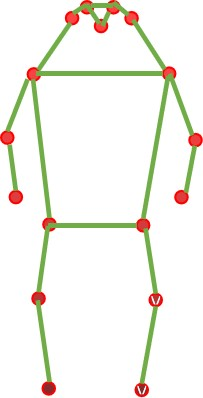
\includegraphics[width=0.5\textwidth]{Figures/keypoints.png}
    \end{minipage}
    \hfill
    \begin{minipage}{0.48\textwidth}
        \centering
        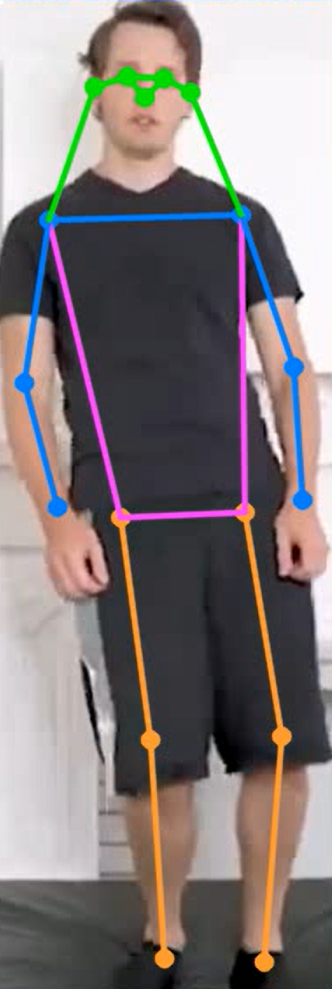
\includegraphics[width=0.35\textwidth]{Figures/pose1.png}
    \end{minipage}
    \caption{(Vlevo) Topologie klíčových bodů použitá např. v COCO-pose.\cite{2dhpe} (Vpravo) Příklad detekce pózy pomocí YOLO.}
    \label{fig:keypoints}
\end{figure}

Úloha detekce pózy spočívá v nalezení klíčových bodů postavy v obraze. Může se
jednat také o zvíře, v našem případě se ale budeme zabývat pouze klíčovými body
lidské postavy. Klíčové body představují důležité body lidského těla, znalost
jejich lokalizace nám umožňuje analyzovat pózu dané osoby, popřípadě sledovat
její pohyb. K základním klíčovým bodům patří hlava, ramena, lokty, zápěstí,
kyčle, kolena a kotníky, viz obrázek \ref{fig:keypoints}. Některé algoritmy dokážou
rozeznat i orientaci dlaně či stopy, nebo rozpoznat klíčové body na hlavě, jako
jsou ústa, nos, oči a uši \cite{blazepose}.

Klíčové body jsou většinou reprezentovány jako dvojice souřadnic $(x, y)$
vzhledem k celému obrazu, některé algoritmy poskytují i souřadnice
normalizované vzhledem k bounding boxu osoby. Existují také algoritmy pro 3D
souřadnice, těmito se ale nebudeme zabývat, i když by mohly stanovit zajímavou
alternativu, zejména pokud by pro detekci bylo použito více kamer z různých
pohledů.

V oblasti algoritmů pro detekci pózy existují dva základní přístupy: zdola
nahoru a shora dolů. Přístup zdola nahoru se snaží detekovat všechny klíčové
body v obraze, aniž by rozlišoval jednotlivé osoby, pokud je algoritmus schopen
detekce pózy pro více osob, pak v dalším kroku tyto body spojuje do
jednotlivých postav. Naproti tomu přístup shora dolů nejprve detekuje všechny
osoby v obraze, v jejich rámci pak detekuje klíčové body.

\section{Detekce klíčových bodů}

U obou výše zmíněných přístupů se nejčastěji provádí vyhledání všech klíčových
bodů pomocí tzv. heatmap. Je to 2D mapa pravděpodobnosti, že se v daném bodě
vyskytuje nějaký klíčový bod. Maximální hodnoty v této mapě pak představují
lokalizaci klíčových bodů.

Pro vygenerování heatmap se používá konvoluční neuronová síť. Pro každý klíčový
bod, resp. pro každý typ klíčového bodu k (v případě detekce pózy více osob)
vzniká jedna heatmapa. Jako referenční heatmapy pro trénování se používají
mapy, kde je klíčový bod reprezentován 2D Gaussovým rozložením s vrcholem v
místě daného bodu.

V dalším kroku jsou z heatmap vygenerovány, nejčastěji s pomocí algoritmu
argmax, souřadnice klíčových bodů. V případě vícero osob je pak třeba tyto body
spojit do jednotlivých osob.

Využití heatmap je velmi přesné, nicméně z důvodu nutnosti provádění dvou
sekvenčních výpočtů je taky trochu pomalé. Některé algoritmy se proto snaží
formulovat úlohu jako regresi vedoucí přímo k souřadnicím klíčových bodů. Tento
přístup je ve své podstatě trochu méně přesný, nicméně je rychlejší.

Vůbec první algoritmus pro detekci pózy využívající hluboké učení, DeepPose
\cite{deeppose}, který byl vytvořen v roce 2014 společností Google, používal
právě tento přístup. Také algoritmus YOLO používá regresi pro určení souřadnic
klíčových bodů, nicméně detekce je prováděná pro detekované objekty, nikoliv
nad celým vstupním obrazem. \cite{yolo-pose}

% , a je součástí poupraveného modelu pro detekci objektů - v posledních
% vrstvách sítě je kromě regrese definující bounding box a klasifikace určující
% třídu prováděna regrese pro určení klíčových bodů.

\section{Detekce objektů a osob v obraze}

Detekce osob se v podstatě může generalizovat na detekci objektů v obraze.
Detekci objektů v obraze definujeme jako úlohu, kdy ve vstupním obrázku určíme
lokaci a třídu všech hledaných objektů.

V kapitole \ref{sec:CNN} jsme si popsali základní architekturu konvolučních
neuronových sítí, ta se ale většinou v praxi používá pro klasifikaci obrázků,
nikoliv pro detekci objektů - algoritmus tedy pouze určí, o jakou třídu objektu
se jedná, a ideálně potřebuje, aby objekt vyplňoval celý vstupní obraz.
Teoreticky by bylo možné detekci formulovat jako regresní problém a natrénovat
takovou síť, která by pomoci několika konvolučních vrstev následovaných
několika plně propojenými vrstvami byla schopna predikovat lokalizaci a třídu
všech objektů v obraze. \cite{szegedy} Problém detekce je ale velice komplexní
a taky by vyžadoval velice komplexní síť - více vrstev s mnoha filtry, resp.
neurony. Jak již ale bylo v zmiňováno, komplexnost sítě zvyšuje její nároky na
výpočetní výkon a komplikuje nebo úplně znemožňuje její trénování s ohledem na
pravděpodobnost přetrénování.

Snahou tedy je najít metody, které poupraví funkčnost sítě tak, aby byla
schopna efektivní detekce objektů. Většina těchto metod se nějakým způsobem
snaží rozdělit vstupní obrázek na menší části, ty následně jednak klasifikovat,
a tedy určit, zda se v dané lokalitě vyskytuje objekt, popřípadě pomocí regrese
určit jeho přesnou lokalizaci. Lokalizace je většinou reprezentována jako
souřadnice obdélníku ohraničujícího daný objekt, tzv. bounding box. Rozdělení
může být provedeno přímo na vstupním obrázku nebo na mapě příznaků v rámci
sítě. Taky můžeme buď rozdělit obrázek na pevně dané oblasti (např. do mřížky)
- jednofázový přístup, anebo v jedné fázi předpřípravit množinu oblastí a ve
druhé fázi nad těmito oblastmi provést klasifikaci a regresi - dvoufázový
přístup.

\subsection{Sliding window}

Jednou z prvních takových metod byl tzv. sliding window (klouzavé okno), který
aplikuje hrubou sílu. Vstupní obrázek se postupně projíždí oknem o fixní
velikosti. Vznikne tak množina pokrývající každou možnou lokaci objektů. Na
tyto oblasti se pak aplikuje klasifikační algoritmus. Postup se opakuje pro
několik velikostí okna, aby se detekovalo objekty různé velikosti.

Tento postup je ale velice pomalý, jelikož je pro každý obrázek zvolený velký
počet oblastí, pro které je třeba provést klasifikaci popřípadě regresi. Navíc
je většina těchto oblastí prázdná, a dochází tak k plýtvání výpočetním výkonem.
Algoritmus se taky potýká s překrývajícími se objekty.

Další metody se tedy snaží redukovat počet oblastí, na které se aplikuje
klasifikace, tak, že se vybere pouze oblasti, které pravděpodobně budou
obsahovat nějaký objekt.

\subsection{Dvoufázový přístup}

\subsubsection{R-CNN}
Prvním algoritmem, který efektivně zredukoval počet oblastí pro klasifikaci,
byl algoritmus R-CNN (Region-based Convolutional Network). \cite{r-cnn} Tento
algoritmus nejprve použil některou z dostupných metod (autoři použili selective
search) pro vygenerování navržených oblastí (region proposals), které
pravděpodobně obsahují nějaký objekt. Tyto metody jsou nezávislé na třídě
objektů. Algoritmus tedy vygeneruje zhruba 2000 oblastí, vzniklé obrázky jsou
následně upraveny na velikost požadovanou CNN v další fázi. CNN extrahuje z
dané oblasti mapu příznaků, na její základě plně propojené vrstvy predikují
třídu objektu popřípadě jeho bounding box.

Problémem R-CNN je, že výběr oblasti a jejich následná klasifikace jsou
nezávislé úlohy a jsou nezávisle trénovány. Detekce objektu je taky poměrně
pomalá, protože je extrakce příznaků prováděná pro všechny oblasti zvlášť. Tyto
problémy se snaží řešit další upravené verze R-CNN.

\subsubsection{Fast R-CNN}
První z nich je Fast R-CNN \cite{fast-r-cnn}, která je upravená tak, aby bylo
možné provádět trénování v jednom kroku. Taky extrahuje příznaky pro celý
vstupní obraz najednou, pomocí selective search pak identifikuje oblasti zájmu
(RoI - Region of Interest), které následně použije pro klasifikaci a regresi.
Tato metoda je přesnější a asi desetkrát rychlejší než původní R-CNN.

\subsubsection{Faster R-CNN}
Další algoritmus, Faster R-CNN \cite{faster-r-cnn}, nahrazuje metodu selective
search vlastní, plně konvoluční sítí RPN (region proposal network).
Zefektivňuje tak proces trénování, výsledná síť je také rychlejší a přesnější
než Fast R-CNN.

\subsection{Jednofázový přístup}

Jednofázový přístup se snaží najít řešení, ve kterém není nutné hledat navržené
oblasti, ale provést klasifikaci a regresi na předem dané množině oblastí,
obvykle určené mřížkou.

\subsubsection{YOLO}
Prvním takovým algoritmem byl YOLO (taky YOLOv1, z ang. you only look once)
\cite{yolo}. Ten, v původní verzi, rozdělí vstupní obraz do pevně dané mřížky
velikosti $S \times S$ a v každém z těchto polí určí $B$ bounding boxů a jejich
třídu. V původní verzi bylo zvoleno $S = 7$ a $B = 2$.

Obraz je nejprve zpracován pomocí konvolučních vrstev, které extrahují mapu
znaků o velikosti $S \times S \times K$, kde $K$ je počet kanálů. Každý pixel
této mapy představuje jedno pole mřížky. Dále je mapa zpracována plně
propojenými vrstvami, které provádějí nad každým polem mřížky klasifikaci a
regresi, viz obrázek \ref{fig:yolo}.

\begin{figure}[]
    \centering
    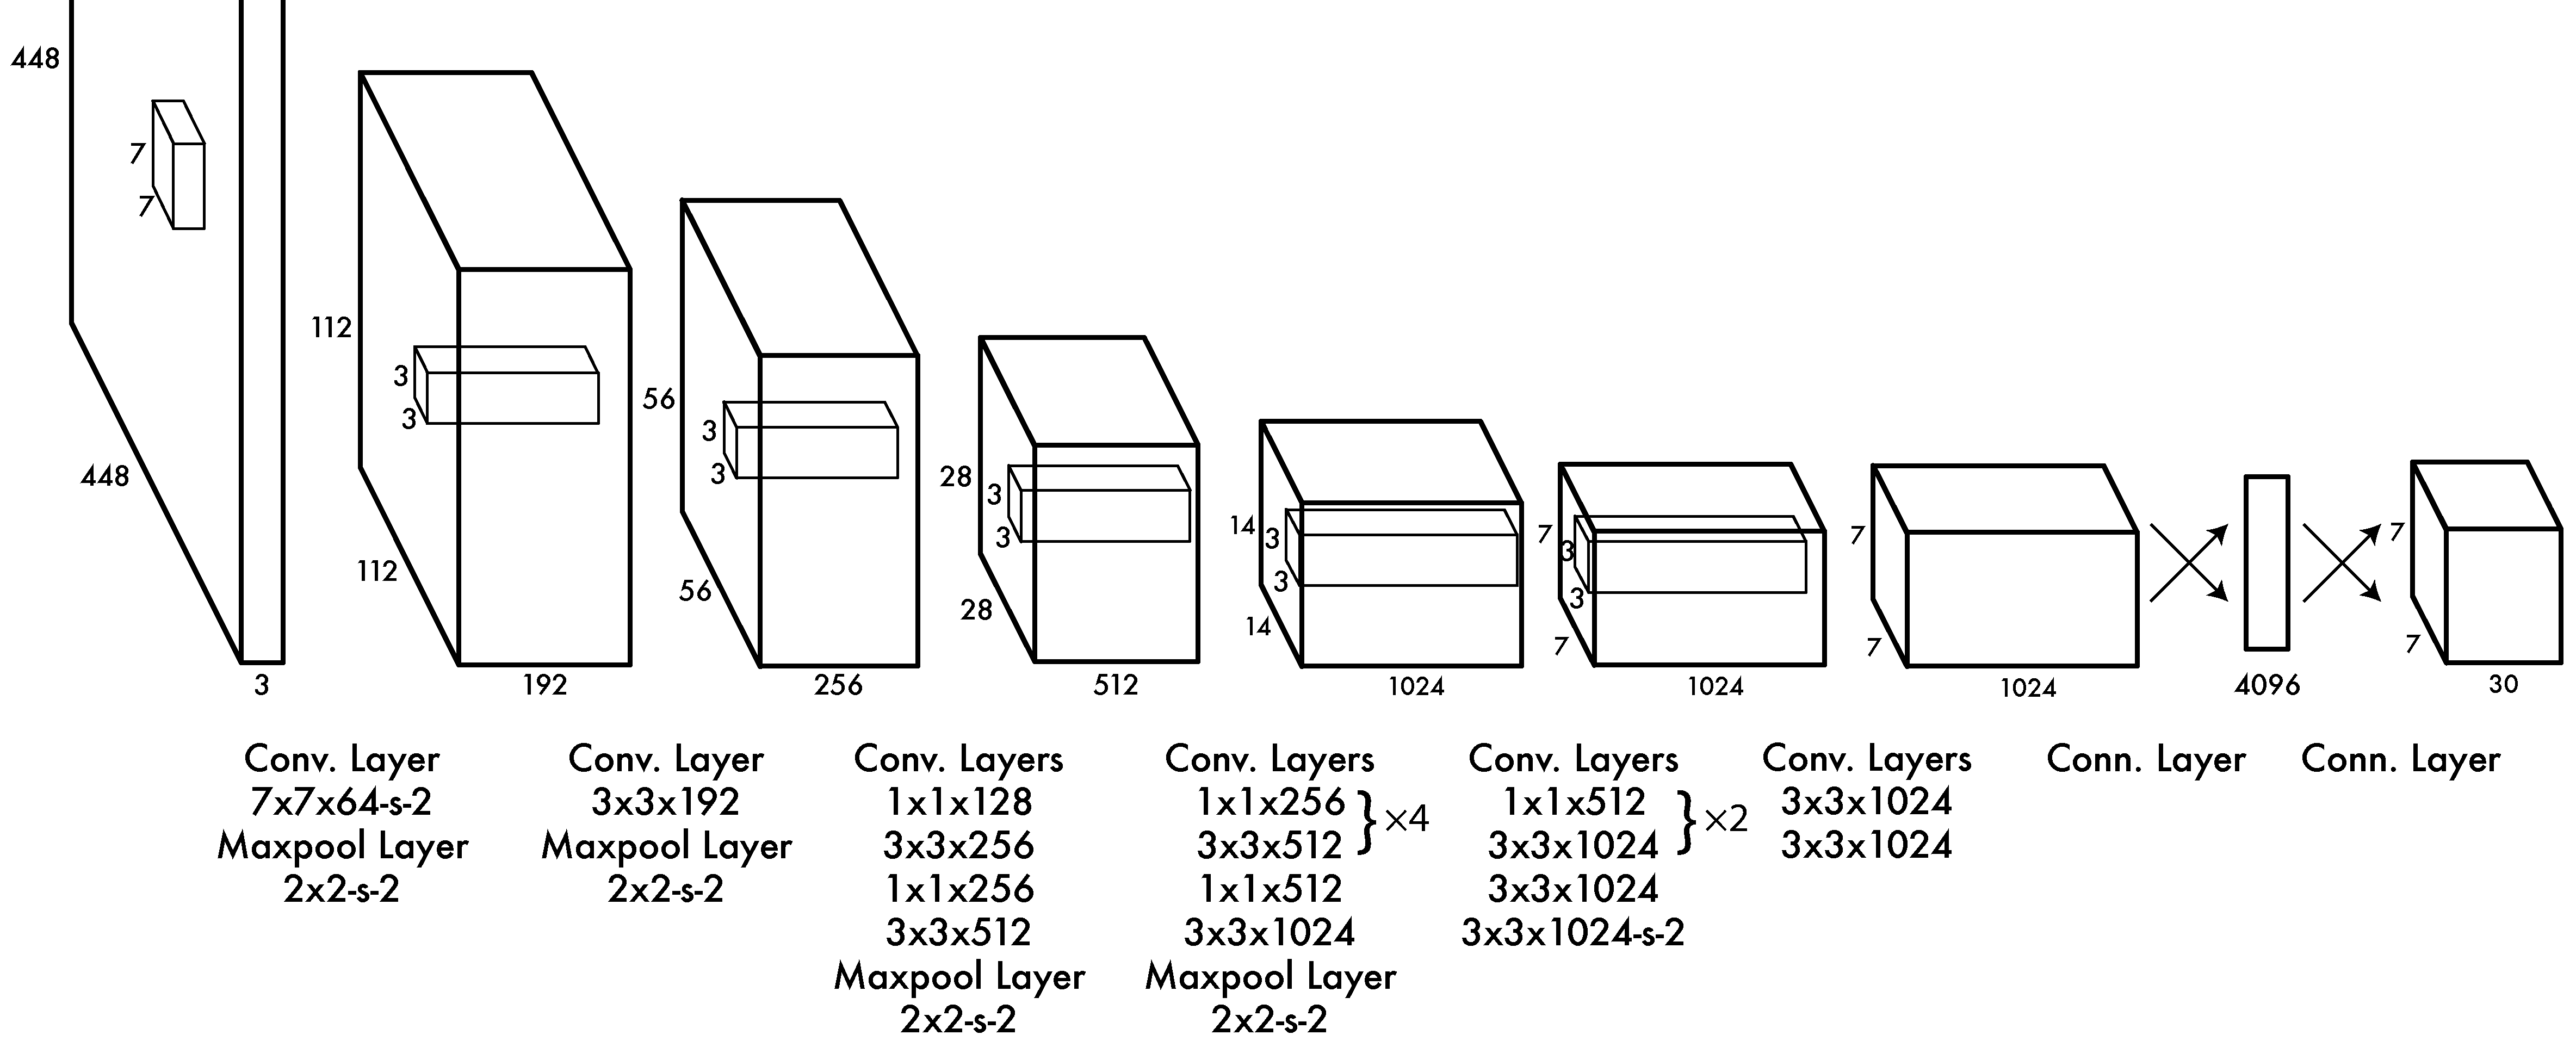
\includegraphics[width=0.8\textwidth]{Figures/yolo}
    \caption{Architektura původní verze YOLO \cite{yolo}}
    \label{fig:yolo}
\end{figure}

Každý bounding box je reprezentován souřadnicemi středu a velikosti (šířka a
výška). Dohromady s informací o jistotě detekce bounding boxu (confidence
score) vrátí model $5$ informací o každém bounding boxu. Pro každé pole mřížky
pak určí společnou informaci o třídě všech objektů v daném poli. Pokud objekt
není detekován, třída indikuje pozadí a souřadnice bounding boxu jsou
ignorovány. Velikost výstupního vektoru je tedy $7 \times 7 \times (2 * 5 +
    C)$, kde $C$ je počet definovaných tříd - v původní verzi pouze 20.

\begin{figure}[]
    \centering
    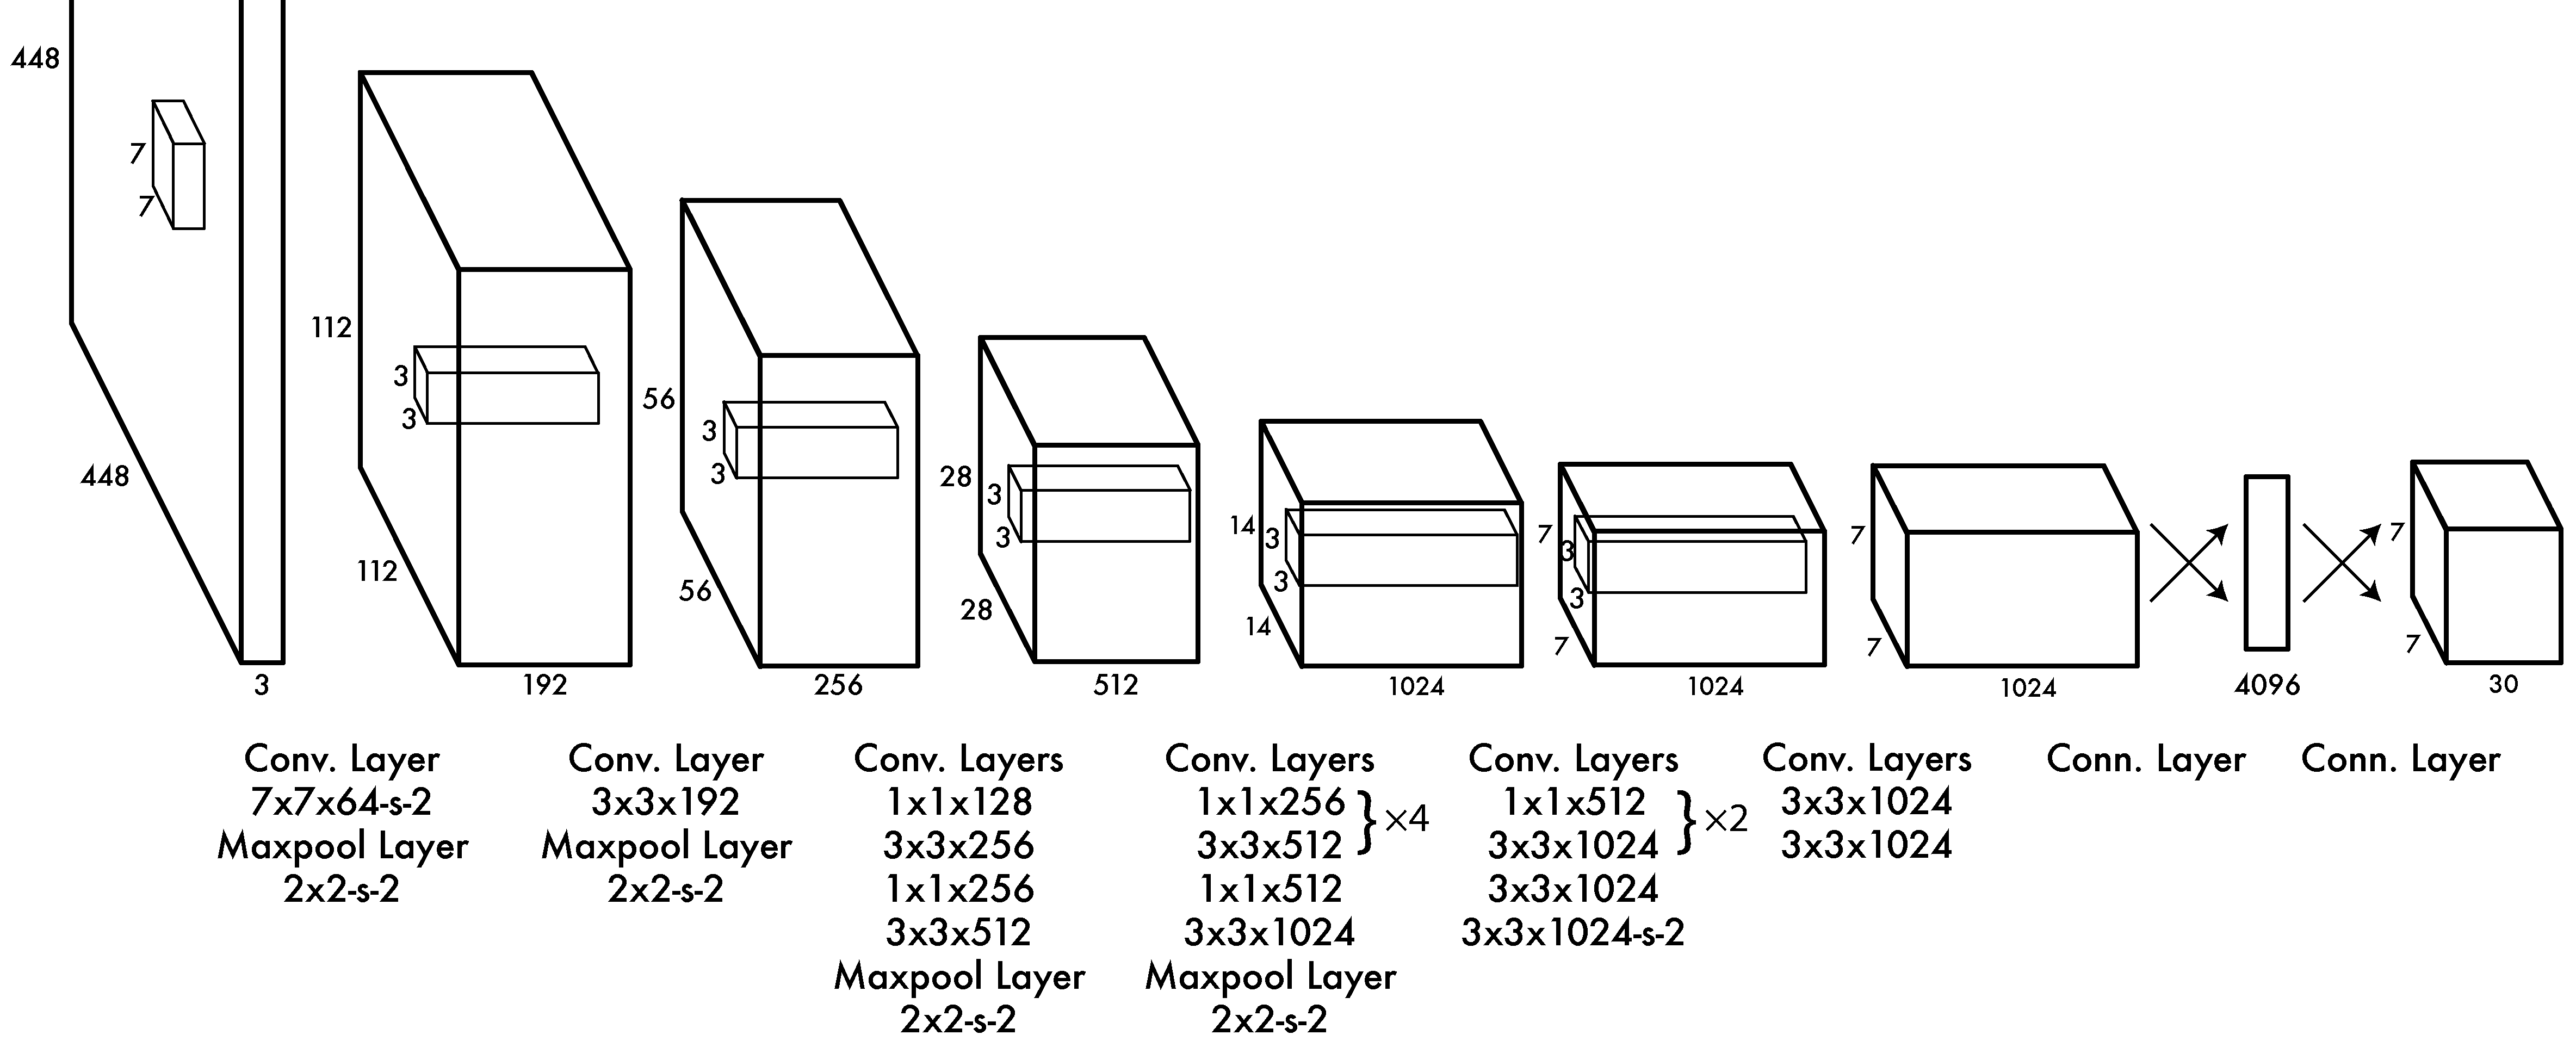
\includegraphics[width=\textwidth]{Figures/yolo}
    \caption{Architektura původní verze YOLO \cite{yolo}}
    \label{fig:yolo}
\end{figure}

Tento algoritmus, navržený v roce 2015 J. Redmonem at al., byl revolučně
rychlý, zároveň v porovnání s jinými real time detekčními algoritmy dosahoval i
slušné přesnosti. Nicméně byl velice citlivý na velikost objektu a přesnost
detekce, zejména u menších objektů, byla horší než u dvoufázových algoritmů.

Další verze algoritmu YOLO přinesly postupná vylepšení ve formě optimalizace
trénování a architektury. YOLOv2 \cite{yolo9000} zavedl mj. trénování na
několika měřítkách a byl natrénován s 9000 třídami (proto taky nazýván
YOLO9000). YOLOv3 \cite{yolov3} přinesl mj. detekci na několika měřítkách.
Postupně byla taky zvětšována mřížka a měnila se použitá architektura CNN sítě
sloužící pro extrakci příznaků pro jednotlivá pole mřížky. Postupně taky byly
přidávány další funkce jako je segmentace, detekce pózy či sledování objektů
(ang. tracking).

V 2020 roce firma Ultralytics poprvé implementovala YOLO s využitím populární
knihovny PyTorch (YOLOv5), což umožnilo snadnější využití YOLO v praxi. Firma
Ultralytics taky vytvořila framework pro použití různých verzí YOLO (YOLOv3 a
novější). Taky pracuje na dalších vylepšeních a optimalizacích. Konkrétně
vytvořila YOLOv5 (2020), YOLOv8 (2023) a YOLOv11 (2024). Tyto verze nicméně
nejsou podloženy odbornými články, někteří je tak považují za neoficiální
verze.

\subsubsection{SSD}
Dalším populárním algoritmem, který používá jednofázový přístup, je SSD (z ang.
single shot detector). \cite{szegedy:ssd} Ten rozdělí vstupní obraz do několika
mřížek o různé velikosti. Postup je takový, že nejprve projde obraz konvoluční
síťí, konkrétně síťí VGG16, která extrahuje mapu příznaků. Tu se postupně
dalšími konvolučními vrstvami zmenšuje, výstup každého stádia zmenšení,
reprezentující mřížku dané velikosti, se spolu s původní mapou dále zpracovává
plně propojenou sítí.
\begin{figure}[]
    \centering
    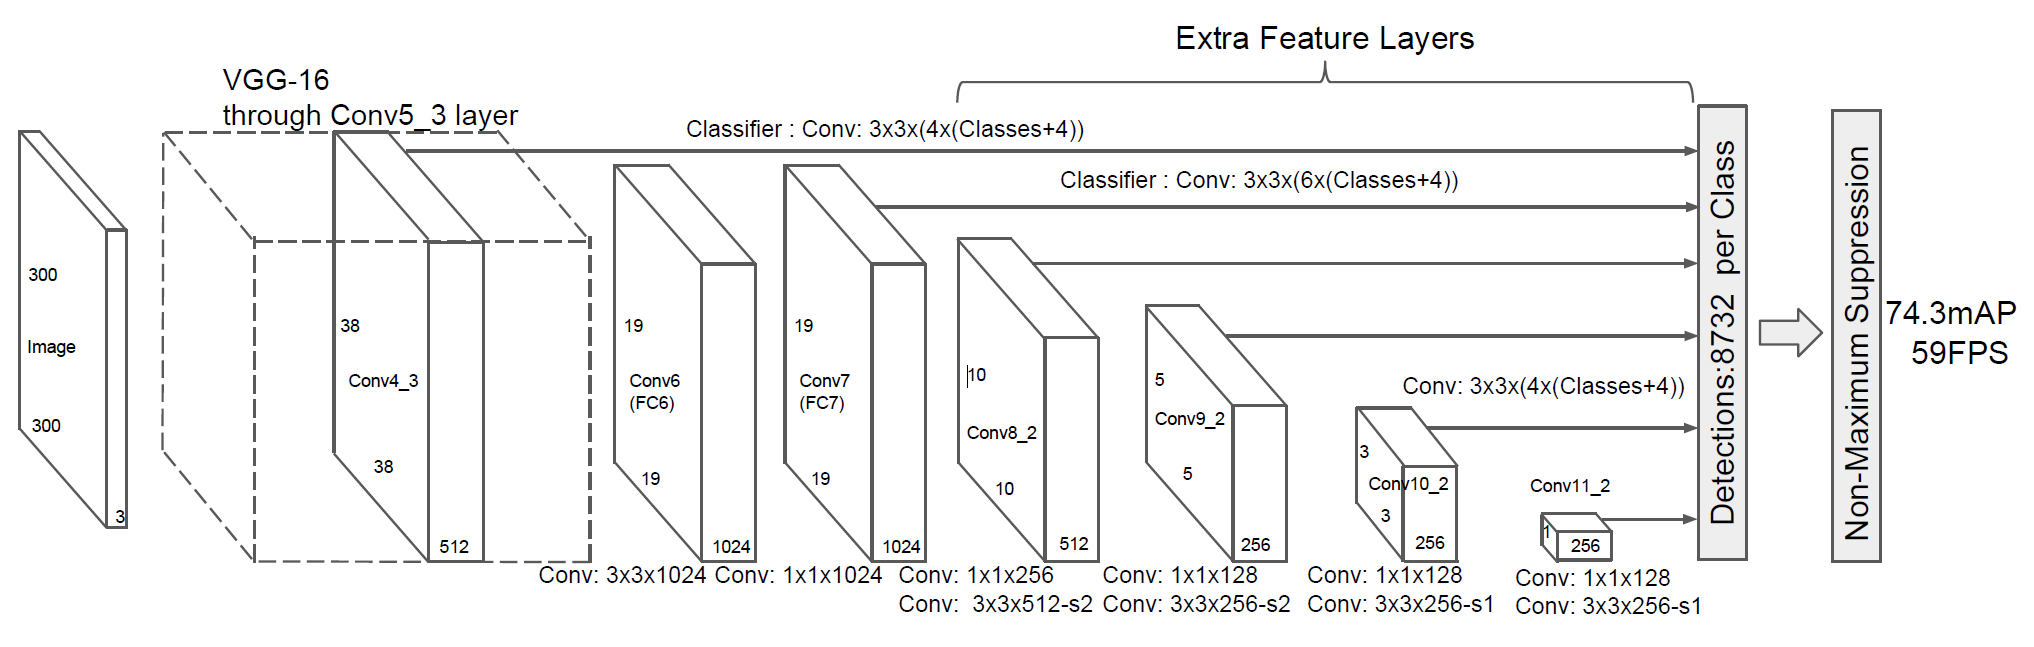
\includegraphics[width=0.8\textwidth]{Figures/ssd.png}
    \caption{Architektura SSD \cite{szegedy:ssd}}
    \label{fig:ssd}
\end{figure}

Výstupní bounding boxy nejsou, jako v případě YOLO, pouze výsledkem regrese,
ale pro každé pole dané mřížky je definováno několik výchozích oblastí (ang.
default box), ze kterých jsou vybrány ty, které obsahují objekt. K ním je
predikována třída objektu a posun i změna velikosti výchozí oblasti,
upřesňující výsledný bounding box.

V době svého vzniku byl SSD rychlejší a přesnější než YOLO, ale novější verze
YOLO jej už předběhly. Nicméně některé principy SSD, jako výchozí oblasti či
použití různých měřítek, byly převzaty do novějších verzí YOLO.

\section{Charakteristiky vybraných algoritmů pro detekci pózy}

V této sekci bude popsáno několik populárních algoritmů pro detekci pózy
zejména se zaměřením na jejich rychlost, přesnost a specifika architektury.

Velká část algoritmů byla zamítnutá a neproběhlo ani jejích testování.
Nejčastějším důvodem zamítnutí některého z algoritmů je, že schází jeho volně
dostupná, aktualizovaná implementace. Tvůrci algoritmů většinou investují čas a
zdroje pro vývoj algoritmu a natrénování modelu (často pro akademické účely),
pak ale neinvestují do jeho údržby. Zejména v prostředí Pythonu, kde se
neustále vyvíjejí nové knihovny a zpětná kompatibilita starších verzí není
zaručena, je pak obtížné použít takovéto řešení ve svém projektu, aniž by bylo
nutné investovat další čas do pochopení zdrojového kódu a jeho úpravy. Jak již
bylo zmíněno na počátku kapitoly, implementace algoritmu od nuly by vyžadovala
velké množství času a zdrojů (zejména výpočetních), hlavně by taky byla
potřebná hlubší znalost problematiky. Někdy je možné řešení použít za cenu
kompromisu ve formě použití starších verzí knihoven či Pythonu, může to ale
představovat bezpečnostní rizika.

\subsection{DeepPose}
DeepPose je historicky první algoritmus pro detekci pózy využívající hluboké
učení. Vyvinuli jej Alexander Toshev a Christian Szegedy ze společnosti Google
v roce 2014. \cite{deeppose} Algoritmus předpokládá, že se ve vstupním obraze
nachází pouze jedná osoba. Síť se snaží v jednom kroku pomocí regrese jak
detekovat osobu, tak i její klíčové body. Jelikož je těžké takto dosáhnout
velmi přesných výsledků, algoritmus používá další fázi, která pomocí regrese
provádí posun bodů k přesnějším výsledkům. Táto fáze je aplikována opakovaně,
kaskádně se tak zvyšuje přesnost detekce.

Při svém vzniku byl DeepPose revoluční, nicméně v porovnání s dnešními řešeními
je poměrně pomalý a nepřesný. Nicméně položil základ pro využití hlubokého
učení v oblasti detekce pózy.

\subsection{OpenPose}

OpenPose \cite{openpose} je typicky příklad přístupu zdola nahoru. Jeho výhodou
je ale možnost vyhledání více osob v jednom snímku. Tento algoritmus, který
vyvinuli v roce 2019 Zhe Cao et al., nejprve pomocí CNN vytvoří heatmapů pro
každý typ klíčového bodu. Pro spojení bodů do jednotlivých osob využije pole
propojení klíčových bodů (ang. part affinity field - PAF). PAF je mapa
vytvořená pro každou končetinu (myšleno obecně spojení dvou klíčových bodů),
která v oblasti dané končetiny obsahuje hodnoty určující směr z jednoho bodu do
druhého. Pokud pak dáme do hromady informace z heatmap a z PAF, jsme schopni
poměrně jednoznačně zkompletovat jednotlivé klíčové body do celých postav.
Stejně jako heatmapy, jsou i PAF součásti trénovacích dat.

\subsection{OpenPifPaf}

Algoritmus OpenPifPaf \cite{openpifpaf}, vyvinutý v roce 2021 Svenem Kreissem
et al., je v podstatě vylepšenou verzi OpenPose. Jeho název je odvozen od dvou
stavebních kamenů: PIF (Part Intensity Field) - pole intenzity klíčových bodů,
a PAF (Part Affinity Field) - pole propojení klíčových bodů. PIF je rozšířením
heatmap, kdy kromě intenzity pravděpodobnosti klíčového bodu obsahuje i jeho
posun, zaručující přesnější lokalizaci bodu, a odhadovanou velikost dané části
těla. PAF v OpenPifPaf je taky podobný tomu v OpenPose, navíc ale indikuje
kromě směru i velikost dané končetiny, což umožňuje lepší prostorové zachycení
pózy.

Dalším rozšířením oproti OpenPose je možnost sledování osob ve videu. Mapa
příznaků, která je výsledkem vstupní CNN, je udržovaná v mězipaměti, do další
části sítě pak vždy vstupují mapy pro aktuální a předchozí snímek. Výstupem pak
kromě klíčových bodů v každém snímku a jejích propojení tvořící kostru, jsou i
propojení mezi klíčovými body z jednotlivých snímků, viz
\ref{fig:pipaf-tracking}. Algoritmus si pak udržuje ID sledovaných osob, pokud
k dříve nalezené osobě je nalezena nová pozice, je jí přiřazeno stejné ID.
Pokud je nalezena nová osoba, je jí přiřazeno nové ID.

\begin{figure}[]
    \centering
    \centering
    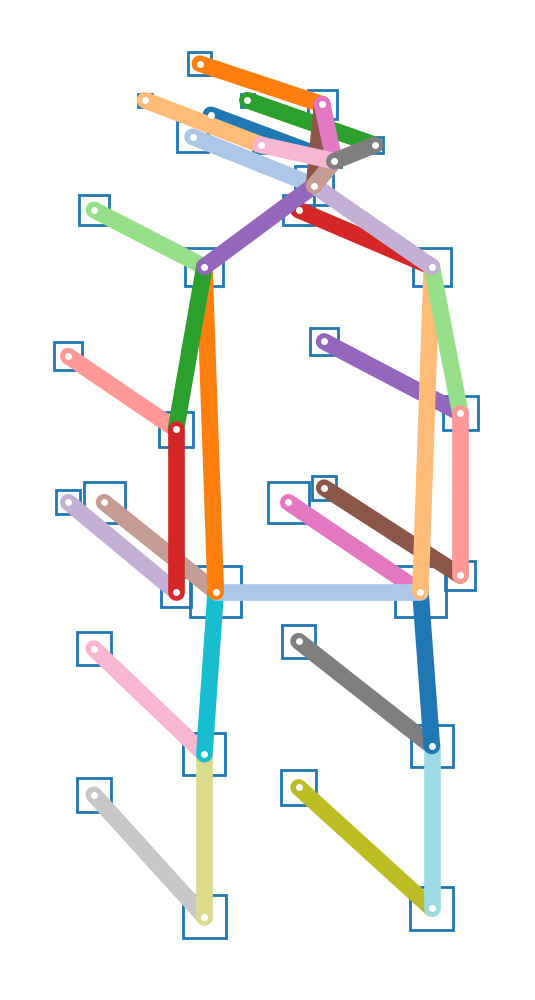
\includegraphics[height=0.2\textheight]{Figures/skeleton_forward2.png}
    \caption{vizualizace  sledování osoby mezi dvěma snímky v OpenPifPaf \cite{openpifpaf}}
    \label{fig:pipaf-tracking}
\end{figure}

\subsection{MediaPipe - BlazePose}

MediaPipe je framework vyvinutý společností Google, umožňujicí jednoduchou
integrací různých technik strojového učení. Obsahuje různé algoritmy pro řešení
úloh jako detekce objektů, segmentace či detekce klíčových bodů (tváře či
pózy). MediaPipe je optimalizován pro mobilní zařízení a webové aplikace.
Detekce pózy v tomto frameworku je postavená na algoritmu BlazePose.

BlazePose implementuje přístup shora dolů, detekuje tedy nejprve oblasti zájmu
(ang. region of interest - RoI), ve kterých detekuje osobu a její pózu. Nativně
podporuje pouze jednu osobu ve snímku. Ve videu ale v rámci optimalizace
neprovádí detekci RoI pro každý snímek, pouze pokud v aktuální RoI již není
detekována osoba. Výhodou tohoto algoritmu je, že detekuje 33 bodů v postavě,
což je podstatně více, než většina ostatních algoritmů, umožňuje tak přesnější
analýzu některých situací, např. podle natočení tváře, dlaní či stop.

Framework MediaPipe implementuje BlazePose spolu z detekcí více osob (použije v
první fáze detektor objektů) i sledování. Výhodou tohoto frameworku je jeho
kontinuální vývoj a jednoduchost integrace. Nevýhodou ale je, že pro systémy
Windows není implementována podpora GPU. Jelikož náš výsledný produkt bude
spouštěn primárně na Windows zařízení, je to pro nás tato vlastnost
rozhodující.

\subsection{Torchvision}

Torchvision je knihovna, která je součástí frameworku PyTorch. Obsahuje různé
nástroje pro strojové vidění, jako je detekce objektů či segmentace. Její
součásti je i předtrénovaný model pro detekci pózy, který je založený na
algoritmu Mask R-CNN.

\subsection{YOLO}

Od vydání YOLOv7 v roce 2022 integruje framework YOLO i detekci pózy. Oficiální
článek Chien-Yao Wanga et al. \cite{yolov7} sice neobsahoval tuto funkčnost,
ale oficiální implementace zahrnula i implementaci YOLO-Pose \cite{yolo-pose}.
Obecně detekce pózy v YOLO kombinuje přístup shora dolů a zdola nahoru.
Algoritmus sice vyhledává klíčové body spolu s bounding boxy osob, nicméně vše
v jednom kroku. Samotná detekce klíčových bodů využívá regresi, což
zjednodušuje proces trénování, jelikož není třeba tvořit heatmapy.

Architektura použita v YOLO-Pose se ale liší od architektury používané v
pozdějších verzích. V YOLO-Pose jsou na konci řetězce umístěny hlavy pro různá
měřítka, jejich výstupem jsou bounding boxy a klíčové body, oba tvořené spolu.
V pozdějších verzích je architektura YOLO koncipována universálněji pro různé
úlohy. Obsahuje tak tři fáze: páteř (ang. backbone), která extrahuje mapu
příznaků, krk (ang. neck), který přizpůsobuje mapu příznaků pro různá měřítka,
a hlavy (ang. head), které paralelně zpracovávají výstupy pro různé úlohy, viz obrázek \ref{fig:yolov11}. 
\cite{yolov11} Bounding box a klíčové body jsou tedy sice generovány paralelně
a teoreticky nezávisle, nicméně s ohledem na proces trénování a postprocessing
se v praxi navzájem výrazně ovlivňují.


\begin{figure}[]
    \centering
    \centering
    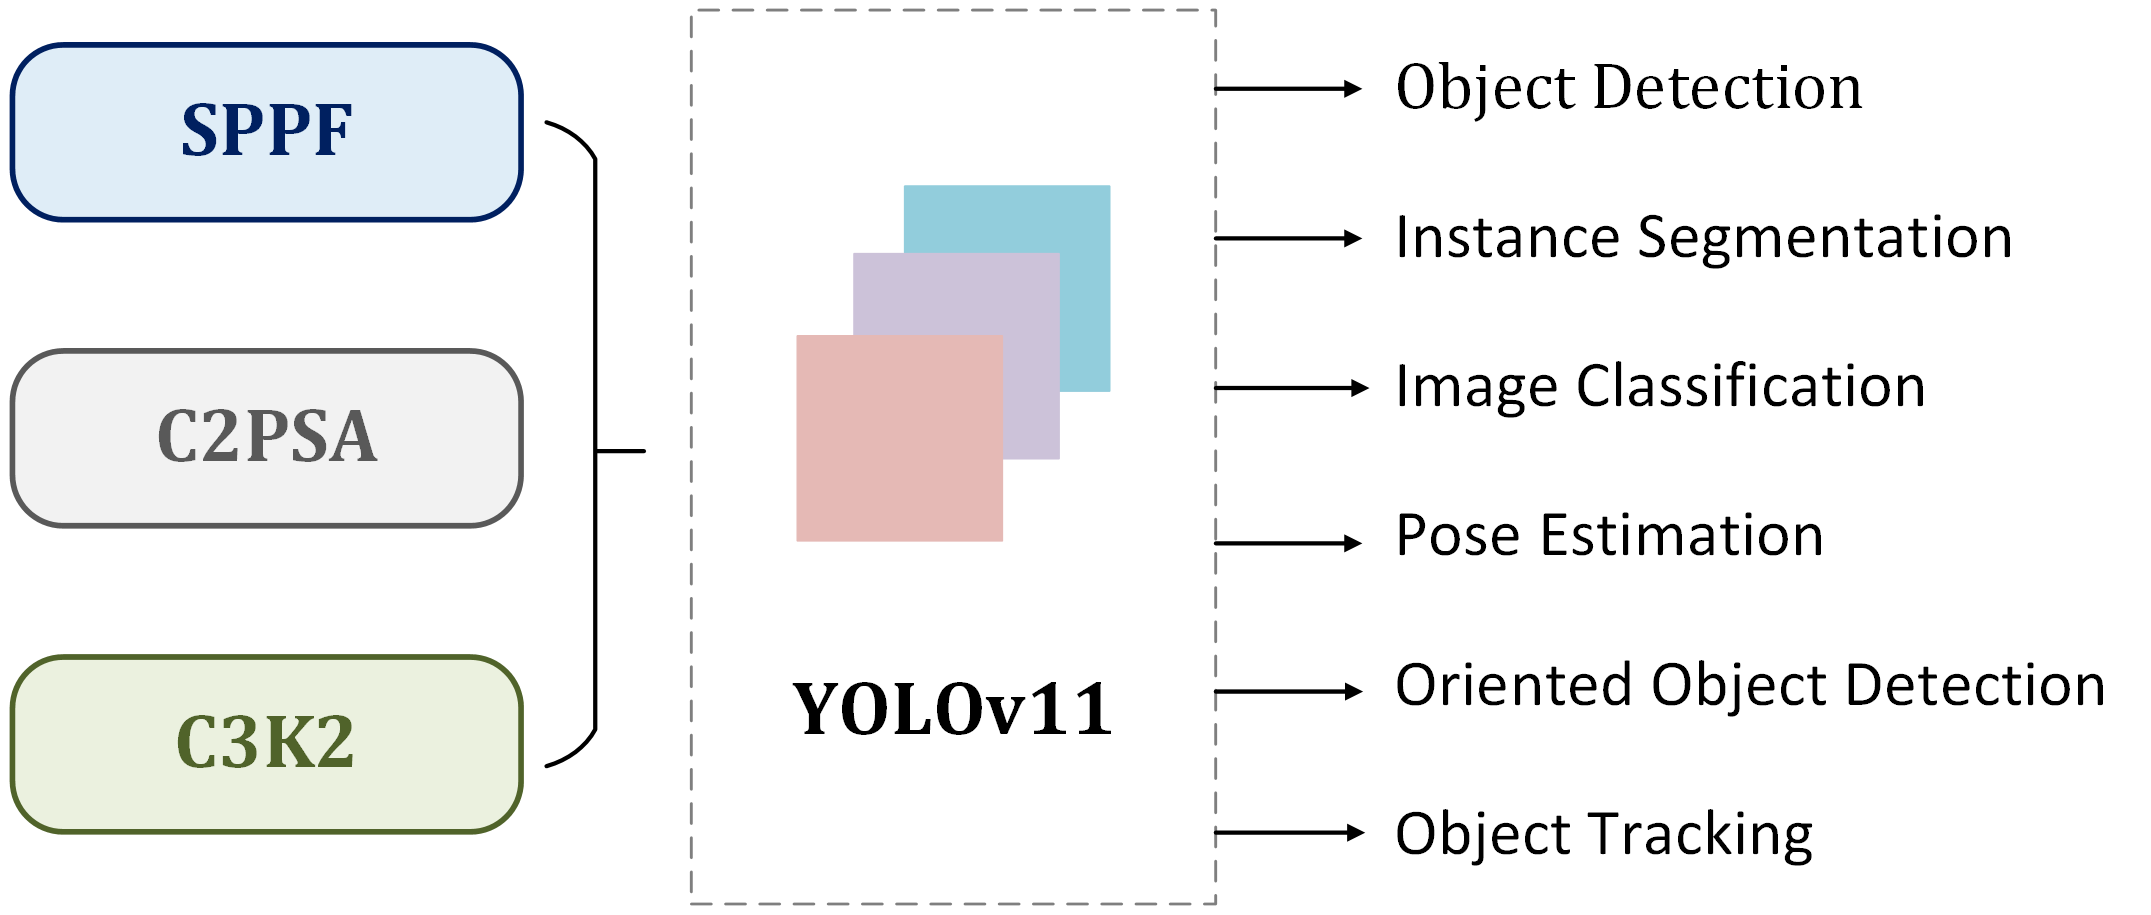
\includegraphics[height=0.2\textheight]{Figures/yolo_v11.png}
    \caption{Architektura YOLOv11 \cite{yolov11}}
    \label{fig:yolov11}
\end{figure}

% openpifpaf, mediapipe(shufflenet, resnet), torchvision, yolo

\endinput